\subsection*{Problema 06}

\noindent\textbf{Enunciado:} \\
Evaluar la integral definida mediante sumas de Riemann y fórmulas de suma:
\begin{align*}
\int_{0}^{2} (3 - x^2) x \, dx
\end{align*}

\noindent\textbf{Solución:} \\
Primero, expandimos el integrando distribuyendo $x$ en la expresión original para obtener un polinomio estándar:
\begin{align*}
(3 - x^2)x &= 3x - x^3
\end{align*}

Sustituyendo esta expansión en la integral definida, la expresión resultante es:
\begin{align*}
I &= \int_{0}^{2} (3x - x^3) \, dx
\end{align*}

Para resolver esta integral mediante sumas de Riemann con el método del extremo derecho, dividimos el intervalo $[0, 2]$ en $n$ subintervalos de igual ancho:
\begin{align*}
\Delta x &= \dfrac{2 - 0}{n} = \dfrac{2}{n}
\end{align*}

Los puntos de partición de la muestra para el extremo derecho son:
\begin{align*}
x_i &= a + i\Delta x = \dfrac{2i}{n}
\end{align*}

Planteamos la integral como el límite de la suma de Riemann:
\begin{align*}
I &= \lim_{n \to \infty} \sum_{i=1}^{n} f(x_i) \Delta x
\end{align*}

Evaluamos la función $f(x) = 3x - x^3$ en $x_i$:
\begin{align*}
f(x_i) &= 3\left(\dfrac{2i}{n}\right) - \left(\dfrac{2i}{n}\right)^{\!3} \\
&= \dfrac{6i}{n} - \dfrac{8i^3}{n^3}
\end{align*}

Multiplicamos por $\Delta x = \dfrac{2}{n}$ y sumamos:
\begin{align*}
f(x_i)\Delta x &= \left(\dfrac{6i}{n} - \dfrac{8i^3}{n^3}\right)\left(\dfrac{2}{n}\right) \\
&= \dfrac{12i}{n^2} - \dfrac{16i^3}{n^4}
\end{align*}

Aplicamos las fórmulas de suma conocidas:
$\sum_{i=1}^{n} i = \dfrac{n(n+1)}{2}$ y 
$\sum_{i=1}^{n} i^3 = \left[\dfrac{n(n+1)}{2}\right]^2$.
Sustituyendo en la sumatoria total:
\begin{align*}
S_n &= \sum_{i=1}^{n} \left(\dfrac{12i}{n^2} - \dfrac{16i^3}{n^4}\right) \\
&= \dfrac{12}{n^2}\sum_{i=1}^{n} i - \dfrac{16}{n^4}\sum_{i=1}^{n} i^3 \\
&= \dfrac{12}{n^2}\left[\dfrac{n^2 + n}{2}\right] \\
&\quad - \dfrac{16}{n^4}\left[\dfrac{n^4 + 2n^3 + n^2}{4}\right]
\end{align*}

Simplificando cada término algebraicamente:
\begin{align*}
S_n &= \left(6 + \dfrac{6}{n}\right) - \left(4 + \dfrac{8}{n} + \dfrac{4}{n^2}\right) \\
&= 2 - \dfrac{2}{n} - \dfrac{4}{n^2}
\end{align*}

Finalmente, calculamos el límite cuando $n \to \infty$:
\begin{align*}
I &= \lim_{n \to \infty} \left(2 - \dfrac{2}{n} - \dfrac{4}{n^2}\right) = 2
\end{align*}

El valor exacto de la integral definida es $2$.

\begin{figure}[H]
	\centering
	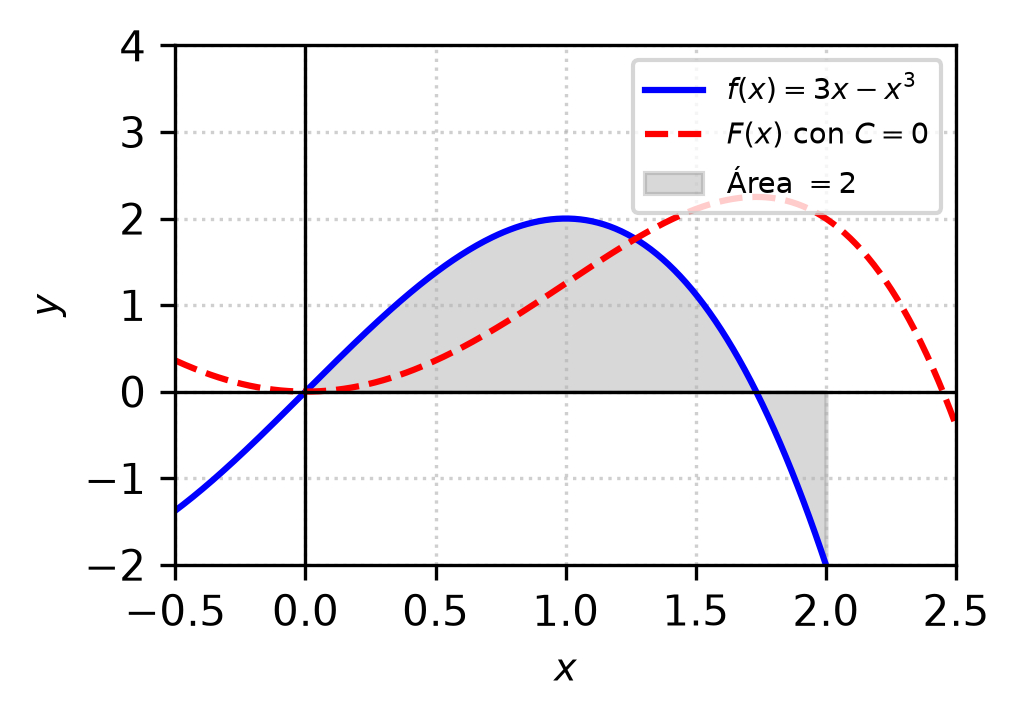
\includegraphics[width=\columnwidth]{semana_06/graficas/SEM06_P06_grafica.png}
	\caption{Representación gráfica de $f(x)$ y su antiderivada $F(x)$ evaluada para la constante de integración $C = 0$ (Problema 06).}
	\label{fig:problema06}
\end{figure}
